\section{Punto de Vista de Realización de resultado}

El punto de vista de la realización de resultados se utiliza para mostrar cómo las capacidades y los elementos básicos subyacentes producen resultados de más alto nivel orientados al negocio.

\subsection{Modelo de Realización de resultado}
\begin{figure}[h!]
	\centering
	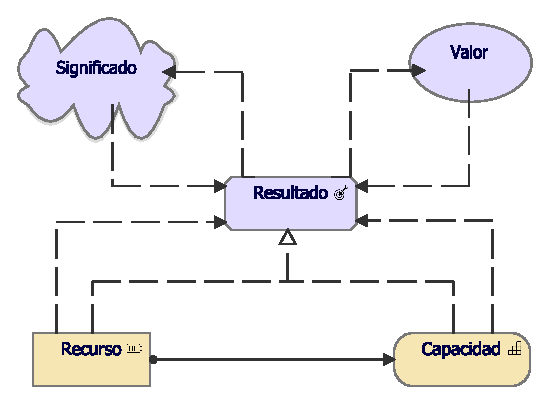
\includegraphics[width=.5\linewidth]{imgs/caso/RealResultado.pdf}
	\caption{Modelo Realización de resultado}
\end{figure}

El punto de vista de la realización de resultados describe cómo las capacidades y los recursos de la empresa producen resultados de alto nivel orientados al negocio.

\newpage

\subsection{Caso de Realización de resultado}

\subsubsection{Resultado 1: Mejores Investigadores e Investigaciones}

\begin{figure}[h!]
	\centering
	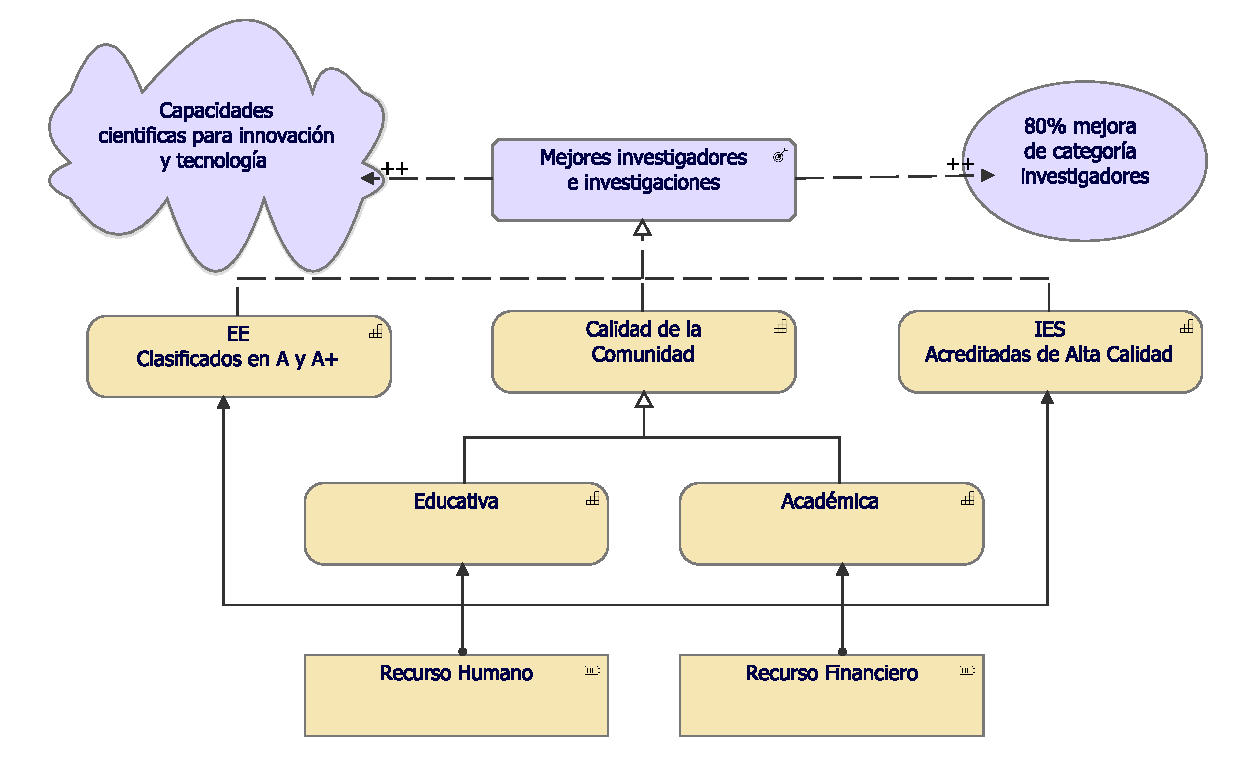
\includegraphics[width=.8\linewidth]{imgs/modelo/estrategia/resultado/resultado_2.pdf}
	\caption{Caso Realización de resultado}
\end{figure}

Para el caso de resultado de \textbf{Mejores Investigadores e Investigaciones} se busca promover nuevas capacidades científicas que fomenten la innovación y la tecnología gracias comunidad de calidad, de las IES acreditadas de alta calidad. Se pretende alcanzar el 80 por ciento en subir de categoría por parte de los investigadores.


\clearpage
\subsubsection{Resultado 2: Generación de Estudiantes de Alta Calidad}

\begin{figure}[h!]
	\centering
	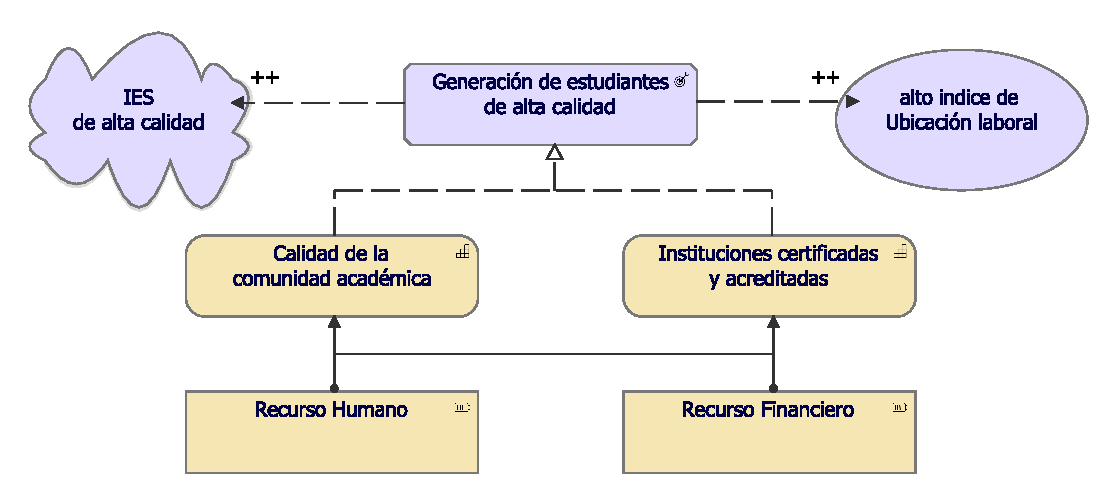
\includegraphics[width=.8\linewidth]{imgs/modelo/estrategia/resultado/resultado.pdf}
	\caption{Caso Realización de resultado}
\end{figure}

El resultado de \textbf{generación de estudiantes de alta calidad} proporciona un significado de grandes expectativas para el MEN, puesto que este resultado da como garantía Instituciones de Educación Superior(IES) de alta calidad promoviendo la capacidad de calidad en la comunidad académica ademas de instituciones certificadas y acreditadas.